\chapter{Engine and ECS Implementation Details}\label{chap:details}

In this chapter, we will go into more detail of how the ECS and game engine are implemented. This includes mostly relevant parts of effect signatures and explanations about the working principles of them.

\newcommand\Boxarray[4]{
  \node[box,fill=#3,minimum height=0.3cm,minimum width=0.3cm] at (#1-0.6,#2) {};
  \node[box,fill=#3,minimum height=0.3cm,minimum width=0.3cm] at (#1-0.3,#2) {};
  \node[box,fill=#3,minimum height=0.3cm,minimum width=0.3cm] (#4) at (#1,#2) {};
  \node[circle,fill=black,inner sep=0cm,minimum height=0.065cm,minimum width=0.065cm] at (#1+0.22,#2) {};
  \node[circle,fill=black,inner sep=0cm,minimum height=0.065cm,minimum width=0.065cm] at (#1+0.3,#2) {};
  \node[circle,fill=black,inner sep=0cm,minimum height=0.065cm,minimum width=0.065cm] at (#1+0.38,#2) {};
  \node[box,fill=#3,minimum height=0.3cm,minimum width=0.3cm] at (#1+0.6,#2) {};
}

\newcommand\Component[3]{
  \node[box,minimum height=1.5cm,minimum width=3.5cm] at (#1,#2) {};
  \node[] at (#1,#2+0.5) {Component[T#3]};
  \node[] at (#1-0.75,#2) {Component ID};
  \node[box,fill=blue!20,minimum height=0.3cm,minimum width=0.3cm] (comp#3id) at (#1+0.75,#2) {};
  \node[] at (#1-0.75,#2-0.5) {Values};
  \Boxarray{#1+0.75}{#2-0.5}{yellow!20}{comp#3arr}
}

\newcommand\Arch[3]{
  \node[box,minimum height=2.5cm,minimum width=5cm,fill=green!20] at (#1,#2) {};
  \node[] at (#1,#2+1) {Arch #3};
  \node[] at (#1-1.5,#2+0.5) {Entities};
  \Boxarray{#1+1.5}{#2+0.5}{yellow!20}{arch#3entarr}
  \node[align=center] at (#1-1.5,#2-0.5) {Component ID\\to indices map};

  \node[box,fill=blue!20,minimum height=0.3cm,minimum width=0.3cm] (arch#3comp1id) at (#1,#2-0.1) {};
  \Boxarray{#1+1.5}{#2-0.1}{purple!20}{arch#3comp1arr}
  \draw[->] (arch#3comp1id.east) -- ([xshift=-0.6cm] arch#3comp1arr.west);

  \node[box,fill=blue!20,minimum height=0.3cm,minimum width=0.3cm] (arch#3comp2id) at (#1,#2-0.5) {};
  \Boxarray{#1+1.5}{#2-0.5}{purple!20}{arch#3comp2arr}
  \draw[->] (arch#3comp2id.east) -- ([xshift=-0.6cm] arch#3comp2arr.west);

  \node[box,fill=blue!20,minimum height=0.3cm,minimum width=0.3cm] (arch#3comp3id) at (#1,#2-0.9) {};
  \Boxarray{#1+1.5}{#2-0.9}{purple!20}{arch#3comp3arr}
  \draw[->] (arch#3comp3id.east) -- ([xshift=-0.6cm] arch#3comp3arr.west);
}

\newcommand\EntityManager[2]{
  \node[box,minimum height=1.5cm,minimum width=4cm] at (#1,#2) {};
  \node[] at (#1,#2+0.5) {EntityManager};
  \node[] at (#1-1,#2) {Entities};
  \Boxarray{#1+1}{#2}{yellow!20}{entarr}
  \node[] at (#1-1,#2-0.5) {Entity Datas};
  \Boxarray{#1+1}{#2-0.5}{purple!20}{entarr}
}

\begin{figure}[h!]
\centering
\tikzstyle{box}=[rectangle,draw,rounded corners=0.5ex,fill=green!10]
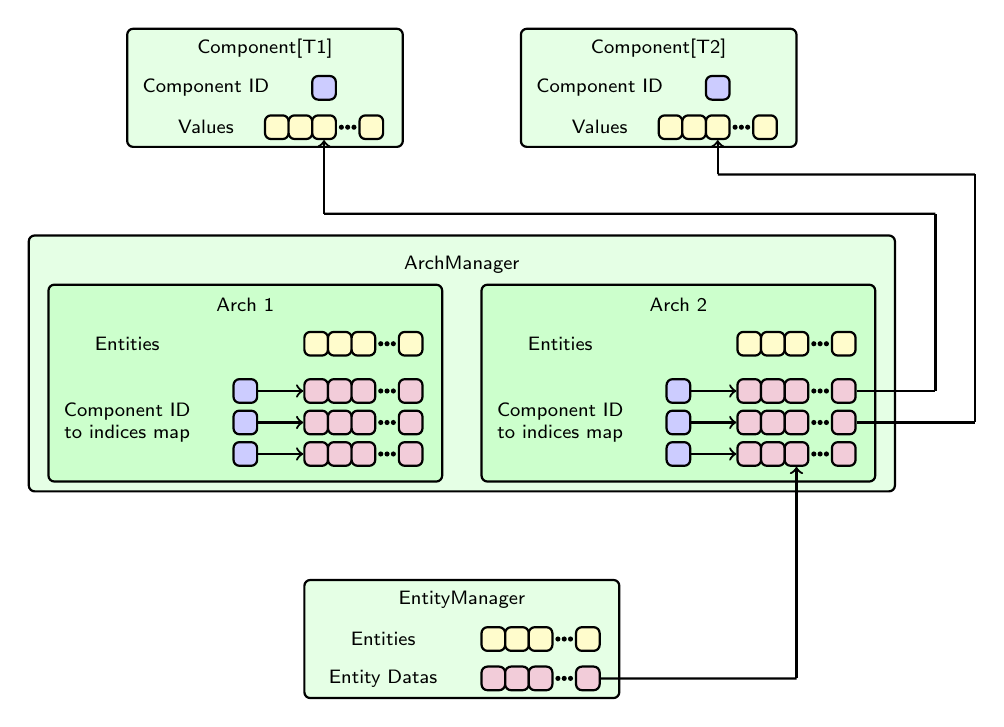
\begin{tikzpicture}[thick,font=\sf\scriptsize]
  \Component{-2.5}{0}{1}
  \Component{2.5}{0}{2}

  \node[box,minimum height=3.25cm,minimum width=11cm] at (0,-3.5) {};
  \node[] at (0,-2.25) {ArchManager};
  \Arch{-2.75}{-3.75}{1}
  \Arch{2.75}{-3.75}{2}
  \draw[-] ([xshift=0.6cm] arch2comp1arr.east) -- ([xshift=1.6cm] arch2comp1arr.east);
  \draw[-] ([xshift=1.6cm] arch2comp1arr.east) -- ([xshift=1.6cm,yshift=2.25cm] arch2comp1arr.east);
  \draw[-] ([xshift=1.6cm,yshift=2.25cm] arch2comp1arr.east) -- ([yshift=-0.935cm] comp1arr.south);
  \draw[->] ([yshift=-0.936cm] comp1arr.south) -- (comp1arr.south);
  \draw[-] ([xshift=0.6cm] arch2comp2arr.east) -- ([xshift=2.1cm] arch2comp2arr.east);
  \draw[-] ([xshift=2.1cm] arch2comp2arr.east) -- ([xshift=2.1cm,yshift=3.15cm] arch2comp2arr.east);
  \draw[-] ([xshift=2.1cm,yshift=3.15cm] arch2comp2arr.east) -- ([yshift=-0.436cm] comp2arr.south);
  \draw[->] ([yshift=-0.436cm] comp2arr.south) -- (comp2arr.south);

  \EntityManager{0}{-7}
  \draw[-] ([xshift=0.6cm] entarr.east) -- ([yshift=-2.686cm] arch2comp3arr.south);
  \draw[->] ([yshift=-2.686cm] arch2comp3arr.south) -- (arch2comp3arr.south);
\end{tikzpicture}
\caption{Simplified internal entity and component storage architecture. Blue boxes are values and multiple boxes arrays, where yellow arrays store values (\textit{Entity} values included) and purple arrays store indices into other arrays. All arrays stacked inside a single box have the same length and corresponding indices (columns). Arrows pointing from values (blue) to arrays represent maps, with the value as key. Arrows from an array of indices pointing to another array indicate which array the first one indexes into.}
\label{fig:effektecs}
\end{figure}

\section{Component Effect and Existentials}\label{sec:compimpl}

A |Component[T]| handler creates a dynamic (resizable) array, containing all the values of that component type without any empty indices. To access a component value (get or set), a component index is used. When a new component is added, it is pushed at the end of the array. Removing an index is done by swapping that value with the last one and popping that last index from the array. This returns the index that was at the end before, so the surrounding/calling code can update the component index of that entity to point to the newly swapped index.

\begin{lstlisting}[caption=Component signature]
interface Component[T] {
  def getComponentId(): Int
  def internalAddComponent(value: T): Int
  def internalSetComponent(index: Int, value: T): Unit
  def internalGetComponent(index: Int): T
  def internalGetComponentStore(): ComponentStore[T]
  def internalCreateSetComponentOp(
    entity: Entity, value: T
  ): SetComponentOp
}
\end{lstlisting}

The engine internals use the component stores of each component type to store all of those values, without separating them by archetype. This can be seen in \Cref{fig:effektecs}. That way, iteration is usually not in order, but it reduces complexity and indirection. Any component value can be easily accessed by using the specific |Component[T]| effect and a component index.

When trying to destroy an entity with multiple components, a major issue occurs. Using the previously mentioned way to remove a component by using the index requires the |Component| effect to be handled, which would need to be done for any component the entity currently has. As dynamic entities were a high priority, meaning any (single) component can be added or removed from an entity dynamically, the component types cannot be stored as part of the type of a component group. This means, the destroy entity operation cannot work by using the |Component| effects of all components the entity has, since that set changes dynamically at runtime.

The solution for this component removal problem is using existential types and a |ComponentManager|. To register any component using the |component| function, the |ComponentManager| needs to be handled, which automatically happens when using the |world| or |engineWorld| setup functions. When a component then creates its component storage variable, it also registers that with the |ComponentManager|, assigning every component type a unique index. It also stores that component storage in an array itself, wrapped in an existential type (|UntypedComponentStore|), making its signature independent of the actual contained component type.

\begin{lstlisting}[caption=ComponentManager signature]
interface ComponentManager {
  def internalRegisterComponentStore[T](
    componentStore: ComponentStore[T]
  ): Int
  def internalRemoveComponent(componentId: Int, index: Int): Unit
}
\end{lstlisting}

When later needing to remove a component, the |ComponentManager| can then be used, together with a component ID and index. Inside that remove operation, the correct component storage is retrieved from an array using the ID and matched on. Inside the match, that index can be removed and swapped with the last index by using the power of existential types:

\begin{lstlisting}
type UntypedComponentStore {
  UntypedComponentStore[T](componentStore: ComponentStore[T])
}
\end{lstlisting}

This works, because the match case knows the type of its component storage, without showing it in its type signature. This way, entities can be destroyed without needing to have any |Component| effect handled at that point:

\begin{lstlisting}
def internalRemoveComponent(componentId, index) = {
  untypedComponentStores.unsafeGet(componentId) match {
    case UntypedComponentStore(componentStore) => {
      componentStore.removeComp(index);
    }
  }
  resume(())
}
\end{lstlisting}

This principle of storing the component data in an existential type also allows setting a component value without the relevant |Component| effect in scope, which is used later for deferred modification in \Cref{sec:entitymanager}.

\section{Archetypes and the ArchManager Effect}

The ECS needs to manage what entities have what components. As it is archetype based, the |ArchManager| effect takes that role. Archetypes define a specific set of component types, so every entity belongs to an archetype and ideally many entities belong to the same archetype. When a component is added or removed from an entity, the entity's archetype changes. The |ArchManager| manages these and stores which entity belongs to which archetype, as seen in \Cref{fig:effektecs}. It creates an archetype whenever an entity gets a component removed or added while its new archetype is not yet present, and removes archetypes that no entity belongs to anymore. In the following signature of |ArchManager|, the return types of most operations are left out for simplicity, as they usually indicate the |EntityData| (arch and component indices) of created/changed and/or swapped entities, so the |EntityManager| can update its database after these operations got called:

\begin{lstlisting}[caption=ArchManager signature]
interface ArchManager {
  def internalHasComponent(archId: Int, componentId: Int): Bool
  def internalAddEntity(entity: Entity): EntityData
  def internalRemoveSwapEntity(
    entityData: EntityData
  ): ...
  def internalGetComponent[T](
    entityData: EntityData
  ): Option[T] / Component[T]
  def internalSetComponent[T](
    entityData: EntityData, value: T,
	componentId: Int, componentStore: ComponentStore[T]
  ): ...
  def internalAddExistingComponent(
    entityData: EntityData, componentId: Int, componentIndex: Int
  ): ...
  def internalRemoveComponent(
    entityData: EntityData, componentId: Int
  ): ...
  ... // Operations for queries to iterate
}
\end{lstlisting}

The |ArchManager| effect acts as the bridge between the |EntityManager| and the actual component values. It has operations to check if a component type is present on a specific entity index, create and destroy entities indices, as well as remove a component from an entity index and add/set or get the value of a component. In its handler, a resizable array is created to hold all |Arch| values, each representing one archetype. Each of those has a map from a component id to a resizable array, which contain all the component indices for the specific component type. Each of these is for one of the entities belonging to this archetype, aligned with a parallel resizable array in the |Arch| containing the actual |Entity| values for iteration.

\section{EntityManager Effect and API}\label{sec:entitymanager}

\textit{Structural changes} is a term often used in ECSs to define changes that do more to the world than modify component values. They include entity creation/destruction, adding components that were not yet present, or removing components from an entity. To summarize: Structural changes are modifications to the world, that may lead to queries needing to recalculate their matches.

Most of the API (interaction from the game developer side) to structurally modify entities and components in the world happens through the |EntityManager| effect. It has operations to check if an entity exists or if it has a specific component type. It can also create and destroy entities, remove components and add/set or get component values.

\begin{lstlisting}[caption=EntityManager signature]
interface EntityManager {
  def hasEntity(entity: Entity): Bool
  def hasComponent[T](
    entity: Entity
  ): Bool / { Component[T], EcsException }
  def createEntity(): Entity
  def destroyEntity(entity: Entity): Unit / EcsException
  def removeComponent[T](
    entity: Entity
  ): Unit / { Component[T], EcsException }
  def getComponent[T](
    entity: Entity
  ): T / { Component[T], EcsException }
  def setComponent[T](
    entity: Entity, value: T
  ): Unit / { Component[T], EcsException }
  ... // Internal operations to get EntityData(s)
}
\end{lstlisting}

The |EntityManager| effect has a second handler implementation that is active inside of system bodies. They handle deferred modification, so that there is no structural modification of the queried component/entity arrays that get iterated over during modification. Newly created entities get reserved without yet being created, so a valid (after the system body) |Entity| value can be returned, which can then be used to add components deferred to the new entity. It forwards calls that can be executed directly to the surrounding normal |EntityManager|, while the commands that should be executed after the system, like creating entities and adding to or removing components from them, need to be executed after the |systemEntityManager| implementation goes out of scope. This can be achieved by calling these operations after the |resume| call, which applies them when the handler goes out of scope. As this is based on a stack, we now have the problem that all operations get applied in reverse order. This means, for example, if the user created an entity and then added a component, it would first try to add the component before the entity exists. This is solved by using the \textit{Command Pattern}, where actions (operations) and all their needed information is stored in objects. The |systemEntityManager| handler creates a list of these operation commands, which every deferred operation call prepends its operation to after the |resume|. Then, at the end of the actual handler's lifetime, all operation commands can be executed in the correct order.

The |EntityManager| effect uses bidirectional effects heavily, as many effects need to be dynamically available at the call site of effect operations instead of the handling site, which is mostly at the start of the game code. Most |EntityManager| operations use the |Component[T]| and |EcsException| effects at call site. This makes all the component types available that have been registered at that point, even after creating the world. The |EcsException| has operations for the error, that the given entity does not exist. It also has one for the specific component type not existing on the given entity, which can be handled for each operation call separately, or the default |panic|ing handler can be used for the whole game.

\section{System Effect}\label{sec:systems}

A |System| represents a single function or code block that gets executed once every frame of the game.

\begin{lstlisting}[caption=System signature]
interface System {
  def internalStep(): Unit / EntityManager
}
\end{lstlisting}

When using the |system| function to add a system to the world, it wraps the current |System| effect handler with a new one, which first calls the body of the existing system and then its own body. This way, nested |System| handlers can be used to create a sequential chain of systems in the order they were added. This whole chain can then get called from the single |step| operation the |System| effect defines. Contextual effect polymorphism is an important feature for systems, as that makes the system code able to use any effect that is in scope where the system is added/defined.

\section{Query Effect}\label{sec:query}

A |Query| effect handler in conjunction with |CompIter| effect handlers can be used to iterate over specific sets of components and their respective |Entity|. This works everywhere the |World| and its requirements are handled, but is mostly used inside systems. Iterating optional components and adding additional filters to require or exclude entities with specific components are also possible with the |Query| implementation.

\begin{lstlisting}[caption=Query and CompIter signatures]
interface Query {
  def addC[T]() {
    prog: { iter: CompIter[T] } => Unit
  }: Unit / Component[T]
  def addOptC[T]() {
    prog: { iter: CompIter[Option[T]] } => Unit
  }: Unit / Component[T]
  def withC[T](): Unit / Component[T]
  def withoutC[T](): Unit / Component[T]
  def foreach() { action: Entity => Unit }: Unit
}

interface CompIter[T] {
  def get(): T
  def set(value: T): Unit
}
\end{lstlisting}

To create a |Query|, the |query| function can be used to define a named handler for the |Query| effect. The |Query| itself can be iterated using the |foreach| operation, which iterates over the current |Entity| value. By calling the |withC| or |withoutC| effect operations on the named |Query| handler, additional filters can be added that do not get iterated themselves. Using the |addC| or |addOptC| effect operations, named handlers of the |CompIter| effect for the respective component can be defined. These can then be used during |Query| iteration to |get| and |set| the specific component value of that type of the current entity, with the respective effect operations.

The |Query| effect also heavily uses bidirectional effects, as the specific |Component[T]| effect must be available at the call site when adding (optional) components or filters to the query.

\section{World Effect and Frame Execution Schedule}

The |World| effect represents the ECS world, but it does very little on its own, as most aspects making up a world are handled by their own effects. The |world| or |engineWorld| functions are mostly there to create all the needed effect handlers.

\begin{lstlisting}[caption=World signature]
interface World {
  def stepWorld(): Unit / System
  def runWorld(): Unit / System
}
\end{lstlisting}

Besides creating all the needed effect handlers in the |world| handler, the |World| effect is responsible for stepping the world a single time with the |stepWorld| effect operation or run it endlessly in a loop with the |runWorld| operation. They both call the current |System| handler's |step| effect operation and in the |runWorld| case then |wait| for the next frame and give control flow back to the JavaScript event loop. The |world| handler also registers the |RunWorld| resource, which is used to exit the endless loop by checking its boolean value every frame.

\section{Canvas Renderer Module}

The |canvasRenderer| is the first and most important module built on top of the ECS to render simple 2D shapes using the HTML5 canvas API. It is essentially a function that adds a |System| to the ECS |World|, as well as handling additional |Component|s and |Resource|s. This working principle is like any other module, including the game developer's actual game code.

\begin{lstlisting}[caption=canvasRenderer signature]
def canvasRenderer() { prog: => Unit / {
  // Provides (handles) resources:
  Resource[Camera], Resource[WindowProperties],
  // Provides (handles) components:
  Component[Shape], Component[DrawHeight],
  // Handles System (needed to add a System):
  System
} }: Unit / {
  // Needs components to be handled:
  Component[Position], Component[Rotation], Component[Scale],
  // Always needed to be handled when adding a System:
  System, EntityIdManager,
  // Generally needed to interact with the ECS:
  ComponentManager, ArchManager, EntityManager, World
}
\end{lstlisting}

The |Camera| and |WindowProperties| resources, as well as the |Shape| and |DrawHeight| components, are created by the |canvasRenderer|. A |Shape| and optional |DrawHeight| component is needed on every entity that should be drawn. The |Shape| type defines the shape (circle, rect, text), as well as containing the color and, for the text shape, the actual text string. The |DrawHeight| defines the drawing order of all the entities, meaning higher values will be drawn in front of shapes with a lower |DrawHeight|. The |Camera| resource defines the position, rotation and height of the camera. The height defines how many size units fit from the bottom to top of the rendered screen area, which could also be called zoom. The |WindowProperties| resource is set by the |canvasRenderer| for the rest of the game logic to read from, if that is needed. It currently only holds the window size in pixels.

The actual drawing happens inside a |System| that gets added to the world, which queries for |Position|s, optional |Rotation|s and |Scale|s, as well as |Shape|s and optional |DrawHeight|s. It inserts all shapes into a binary min-|Heap| based on their draw height, so they can be drawn from back to front using the |deleteMin| function from the heap. Before rendering, the canvas is first transformed to make its height exactly one size unit, after which the |Camera|'s transform is applied, to offset, rotate and zoom the canvas based on the |Camera|'s parameters. For each shape, the current canvas transformation is first saved. The canvas is then transformed again based on the |Shape|'s position, rotation and scale, after which the shape can always be drawn in the center with unit dimensions (size of one). After rendering a shape, the transform from before the shape, but after the camera transform is restored again.

Interfacing with the canvas is implemented by using the \textit{ffi} (foreign function interface), where each function needed on the canvas has an |external| JavaScript definition. The canvas itself is also defined as an |extern type|, to be able to pass it to the external functions.

\section{Player Input Module}

The player input is not handled in Effekt so far, only interfaced with the \textit{ffi}. This could be changed with JavaScript to Effekt callbacks, but that would need further consideration. Also, it currently only supports keyboard input, no mouse or gamepads.

In the external JavaScript implementation, all key events are captured and pushed into sets, which get reset every frame. One set is for the keys that were pressed in this frame and one for the released keys. A third set holds all keys that are currently held down, so these only get removed when the respective key release event is received. With \textit{ffi} functions, any Effekt code can check a specific key (identified by JavaScript |KeyCode|) for currently being pressed, just pressed this frame or released this frame.
